\documentclass[11pt,a4paper]{article}

\usepackage[T1]{fontenc}
\usepackage[utf8]{inputenc}
\usepackage{amsmath}
\usepackage{newtxtext,newtxmath}
\usepackage[varqu]{zi4}
\usepackage{microtype}
\usepackage[margin=1in]{geometry}
\usepackage{array,booktabs,tabularx,longtable}
\usepackage[dvipsnames]{xcolor}
\usepackage{tikz}
\usetikzlibrary{positioning,arrows.meta,calc,decorations.pathreplacing}
\usepackage[font=small,labelfont=bf]{caption}
\usepackage{enumitem}
\usepackage{needspace}
\usepackage{listings}
\lstset{basicstyle=\ttfamily\footnotesize, columns=fullflexible, keepspaces,
  morecomment=[l]{;}, commentstyle=\color{black!55}, frame=single,
  rulecolor=\color{black!30}, xleftmargin=4pt, xrightmargin=4pt,
  aboveskip=8pt, belowskip=8pt}
\lstdefinestyle{shell}{morecomment=[l]{\#}, frame=none, backgroundcolor=\color{black!4}}
\usepackage[colorlinks,linkcolor=MidnightBlue,urlcolor=MidnightBlue]{hyperref}
\usepackage[nameinlink]{cleveref}

\newcommand{\vm}{VM16}
\newcommand{\op}[1]{\texttt{#1}}
\newcommand{\hx}[1]{\texttt{0x#1}}
\newcommand{\mw}{\mathrm{mem}_{16}}
\newcommand{\mb}{\mathrm{mem}_{8}}
\newcommand{\sx}{\mathrm{sext}}
\newcommand{\R}[1]{r_{#1}}

\definecolor{opc}{HTML}{FCE8D2}
\definecolor{regc}{HTML}{DCE9F7}
\definecolor{immc}{HTML}{DDF0DC}

\tikzset{>=Stealth, every picture/.append style={font=\small}}

\setlength{\parskip}{3pt}

\title{\vm{}: A Minimal Portable 16-bit Virtual Machine\\[4pt]
\large Specification, version 0.1 (draft)}
\author{}
\date{\today}

\begin{document}
\maketitle

\begin{abstract}
\noindent
\vm{} is a small register-and-stack virtual machine meant to be implemented
in a few hundred lines of assembly language on 8- and 16-bit processors such as
the Z80, 6502 and 8086. It is powerful enough to write a memory allocator, a
garbage collector, hash tables, and an interpreter for a higher-level abstract
machine such as an SECD machine or a combinator graph reducer. This document
defines the machine state, the instruction encoding, the exact semantics of
every instruction, the system-call interface and the program image format. A
recommended calling convention and assembly syntax are given as non-normative
appendices.
\end{abstract}

\tableofcontents

% =====================================================================
\section{Goals and principles}

\begin{enumerate}[label=\textbf{P\arabic*.}, leftmargin=2.2em]
\item \textbf{Small to implement.} An interpreter should fit in 1--2\,KB of
  native code on an 8-bit processor. Every instruction has a fixed,
  simple decoding.
\item \textbf{Identical on every host.} The semantics never depend on host
  flags, word size or byte order. There is no flags register: conditional
  branches compare registers directly.
\item \textbf{Untyped.} The machine knows words, bytes and addresses only.
  Heap allocation, garbage collection, tagging and data structures are
  written in \vm{} code, as libraries.
\item \textbf{Precise roots.} Return addresses live on a return stack
  separate from the data stack, so a garbage collector written in \vm{} code
  can scan the data stack without mistaking a return address for a pointer.
\item \textbf{Good for writing interpreters.} Indirect jumps and calls
  through registers support jump-table dispatch.
\item \textbf{An escape hatch.} The \op{SYS} instruction gives access to host
  services and to native implementations of performance-critical routines.
\end{enumerate}

\paragraph{Conventions.} The key words \emph{must}, \emph{must not} and
\emph{may} are normative. Numbers written \hx{1F} are hexadecimal. All
arithmetic on addresses and register values is modulo $2^{16}$.

% =====================================================================
\section{Machine state}\label{sec:state}

\begin{figure}[h]
\centering
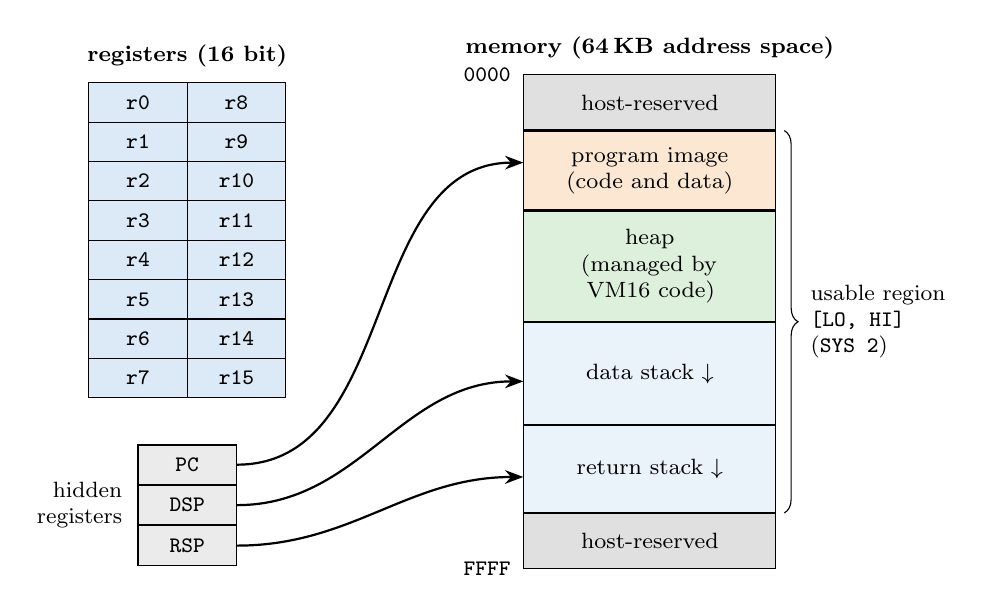
\begin{tikzpicture}[
  reg/.style={draw, fill=regc, minimum width=1.25cm, minimum height=0.5cm, font=\footnotesize\ttfamily},
  hid/.style={draw, fill=black!8, minimum width=1.25cm, minimum height=0.5cm, font=\footnotesize\ttfamily},
  mem/.style={draw, text width=3.0cm, inner xsep=0.1cm, align=center, font=\footnotesize},
]
% register file: 2 columns of 8
\foreach \i in {0,...,7} {
  \node[reg] (ra\i) at (0, -0.5*\i) {r\i};
  \pgfmathtruncatemacro{\j}{\i+8}
  \node[reg] (rb\i) at (1.25, -0.5*\i) {r\j};
}
\node[font=\bfseries\footnotesize, above=2pt of $(ra0.north)!0.5!(rb0.north)$] {registers (16 bit)};
\node[hid] (pc) at (0.625,-4.6) {PC};
\node[hid, below=0pt of pc] (dsp) {DSP};
\node[hid, below=0pt of dsp] (rsp) {RSP};
\node[font=\footnotesize, left=2pt of dsp, align=right] {hidden\\registers};
% memory strip
\node[mem, fill=black!12, minimum height=0.7cm] (m0) at (6.5,0.0) {host-reserved};
\node[mem, fill=opc, minimum height=1.0cm, below=0pt of m0] (m1) {program image\\ (code and data)};
\node[mem, fill=immc, minimum height=1.4cm, below=0pt of m1] (m2) {heap\\ (managed by \vm{} code)};
\node[mem, fill=regc!60, minimum height=1.3cm, below=0pt of m2] (m3) {data stack $\downarrow$};
\node[mem, fill=regc!60, minimum height=1.1cm, below=0pt of m3] (m4) {return stack $\downarrow$};
\node[mem, fill=black!12, minimum height=0.7cm, below=0pt of m4] (m5) {host-reserved};
\node[font=\bfseries\footnotesize, above=2pt of m0] {memory (64\,KB address space)};
\node[font=\footnotesize\ttfamily, left=1pt of m0.north west, anchor=east] {0000};
\node[font=\footnotesize\ttfamily, left=1pt of m5.south west, anchor=east] {FFFF};
\draw[decorate, decoration={brace, amplitude=5pt}] ($(m1.north east)+(0.1,0)$) -- node[right=6pt, font=\footnotesize, align=left] {usable region\\ \texttt{[LO, HI]}\\ (\op{SYS 2})} ($(m4.south east)+(0.1,0)$);
\draw[->, thick] (pc.east) to[out=0, in=180] ($(m1.west)+(0,0.1)$);
\draw[->, thick] (dsp.east) to[out=0, in=180] ($(m3.west)+(0,-0.1)$);
\draw[->, thick] (rsp.east) to[out=0, in=180] ($(m4.west)+(0,-0.1)$);
\end{tikzpicture}
\caption{The \vm{} machine state. The register file is not part of the
address space. The layout of the usable region shown here is only an example:
the program image header (\cref{sec:image}) chooses where the stacks start, and
the program decides where its heap lives.}
\label{fig:state}
\end{figure}

\subsection{Registers}

\begin{itemize}
\item Sixteen general-purpose 16-bit registers $\R{0},\dots,\R{15}$. No
  register has a special meaning to the hardware, except that \op{DIVU}
  writes its remainder to $\R{15}$.
\item Three hidden 16-bit registers: the program counter PC, the data stack
  pointer DSP and the return stack pointer RSP. They are read and written only
  by the instructions that name them.
\item The register file is \emph{not} mapped into the address space. An
  implementation may keep it anywhere, for example in 6502 zero page.
\end{itemize}

\subsection{Memory}

\begin{itemize}
\item Memory is an array of $2^{16}$ bytes. A \vm{} address is used directly as a host
  address (identity mapping), so an implementation never has to translate
  addresses.
\item Not all of it is available to the program: the host needs room for the
  interpreter, I/O and its own stack. The \emph{usable region} is the
  contiguous range $[\mathrm{LO}, \mathrm{HI}]$ reported by \op{SYS 2}. A
  program must not read or write outside it. Doing so is undefined behaviour
  (\cref{sec:ub}).
\item Words are 16 bits, little-endian, and need not be aligned:
  \[
    \mw(a) = \mb(a) + 256\cdot\mb(a+1 \bmod 2^{16}).
  \]
  Storing a word writes the low byte at $a$ and the high byte at $a+1$.

  \emph{Example.} Suppose the byte at \hx{0302} is \hx{AB}, and $\R{2} = \hx{0300}$.
  \begin{center}
  \small
  \begin{tabular}{@{}l l@{}}
  \op{LI r1, 0x1234} & \\
  \op{SW r1, [r2+0]} & writes \hx{34} at \hx{0300} and \hx{12} at \hx{0301}\\
  \op{LW r3, [r2+0]} & $\R{3} = \hx{34} + 256\cdot\hx{12} = \hx{1234}$\\
  \op{LW r4, [r2+1]} & unaligned: $\R{4} = \hx{12} + 256\cdot\hx{AB} = \hx{AB12}$\\
  \op{LB r5, [r2+0]} & $\R{5} = \hx{0034}$, the low byte only\\
  \end{tabular}
  \end{center}
  \vspace{-2pt}
  \begin{center}
  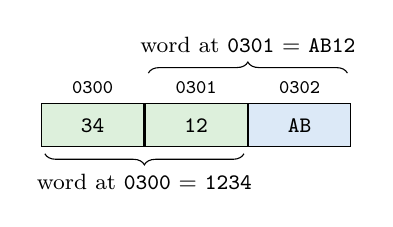
\begin{tikzpicture}[byte/.style={draw, minimum width=1.3cm, minimum height=0.55cm, font=\footnotesize\ttfamily}]
  \node[byte, fill=immc] (b0) at (0,0) {34};
  \node[byte, fill=immc, right=0pt of b0] (b1) {12};
  \node[byte, fill=regc, right=0pt of b1] (b2) {AB};
  \foreach \n/\a in {b0/0300, b1/0301, b2/0302} {\node[font=\scriptsize\ttfamily, above=0pt of \n] {\a};}
  \draw[decorate, decoration={brace, mirror, amplitude=4pt}] ($(b0.south west)+(0.05,-0.08)$) -- node[below=4pt, font=\footnotesize] {word at \texttt{0300} = \texttt{1234}} ($(b1.south east)+(-0.05,-0.08)$);
  \draw[decorate, decoration={brace, amplitude=4pt}] ($(b1.north west)+(0.05,0.38)$) -- node[above=4pt, font=\footnotesize] {word at \texttt{0301} = \texttt{AB12}} ($(b2.north east)+(-0.05,0.38)$);
  \end{tikzpicture}
  \end{center}
  Addresses wrap around: the word at \hx{FFFF} consists of the bytes at
  \hx{FFFF} (low) and \hx{0000} (high).
\item Code and data share one memory. A store that modifies an instruction
  takes effect the next time that instruction is fetched. Programs that rely
  on this are not portable to implementations that translate \vm{} code to
  native code (\cref{app:notes}).
\end{itemize}

\subsection{Stacks}

Both stacks live in memory, grow towards lower addresses, and are \emph{full
descending}: the stack pointer holds the address of the item most recently
pushed. Each item is one word.
\[
\begin{array}{@{}ll@{}}
\text{push } v: & \mathit{SP} \gets \mathit{SP}-2;\ \ \mw(\mathit{SP}) \gets v\\
\text{pop:} & v \gets \mw(\mathit{SP});\ \ \mathit{SP} \gets \mathit{SP}+2
\end{array}
\]
The machine does not check for overflow or underflow. It is up to the program
image to give each stack enough room.

\subsection{Initial state}

When a program image is loaded (\cref{sec:image}), PC, DSP and RSP are taken
from the image header, all of $\R{0},\dots,\R{15}$ are zero, and memory outside the image
is unspecified.

% =====================================================================
\section{Instruction encoding}\label{sec:encoding}

Every instruction begins with a one-byte \emph{opcode}, followed by zero to
three operand bytes. There are eight formats (\cref{fig:formats}).

\begin{figure}[h]
\centering
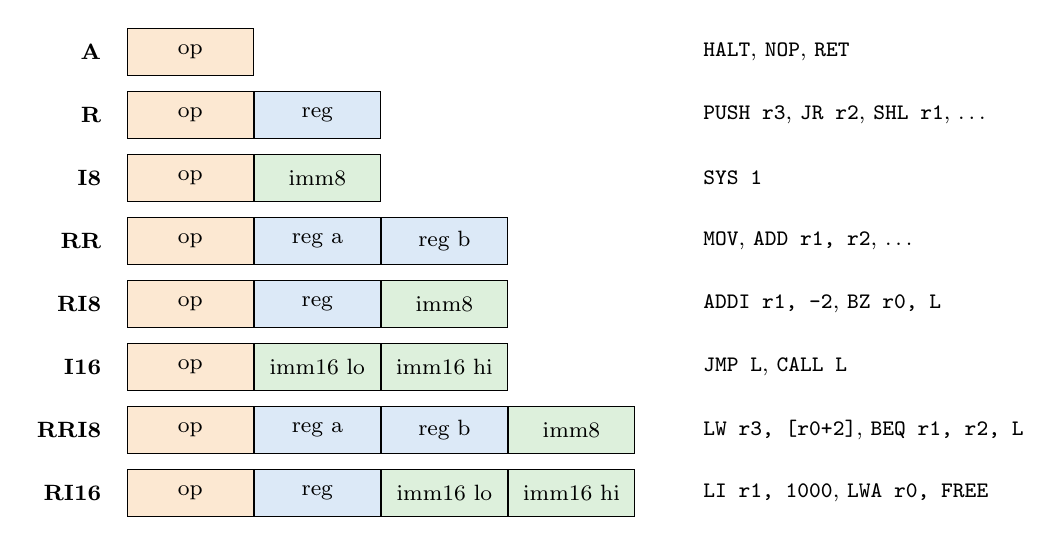
\begin{tikzpicture}[
  b/.style={draw, minimum width=1.6cm, minimum height=0.6cm, font=\footnotesize},
  o/.style={b, fill=opc}, r/.style={b, fill=regc}, i/.style={b, fill=immc},
  fmt/.style={anchor=east, font=\footnotesize\bfseries},
  ex/.style={anchor=west, font=\footnotesize}]
\newcommand{\row}[3]{\node[fmt] at (-0.2,#1) {#2}; \node[ex] at (7.2,#1) {#3};}
\row{0}{A}{\op{HALT}, \op{NOP}, \op{RET}}
\node[o, anchor=west] at (0,0) {op};
\row{-0.8}{R}{\op{PUSH r3}, \op{JR r2}, \op{SHL r1}, \dots}
\node[o, anchor=west] (x) at (0,-0.8) {op}; \node[r, right=0pt of x] {reg};
\row{-1.6}{I8}{\op{SYS 1}}
\node[o, anchor=west] (x) at (0,-1.6) {op}; \node[i, right=0pt of x] {imm8};
\row{-2.4}{RR}{\op{MOV}, \op{ADD r1, r2}, \dots}
\node[o, anchor=west] (x) at (0,-2.4) {op}; \node[r, right=0pt of x] (y) {reg a}; \node[r, right=0pt of y] {reg b};
\row{-3.2}{RI8}{\op{ADDI r1, -2}, \op{BZ r0, L}}
\node[o, anchor=west] (x) at (0,-3.2) {op}; \node[r, right=0pt of x] (y) {reg}; \node[i, right=0pt of y] {imm8};
\row{-4.0}{I16}{\op{JMP L}, \op{CALL L}}
\node[o, anchor=west] (x) at (0,-4.0) {op}; \node[i, right=0pt of x] (y) {imm16 lo}; \node[i, right=0pt of y] {imm16 hi};
\row{-4.8}{RRI8}{\op{LW r3, [r0+2]}, \op{BEQ r1, r2, L}}
\node[o, anchor=west] (x) at (0,-4.8) {op}; \node[r, right=0pt of x] (y) {reg a}; \node[r, right=0pt of y] (z) {reg b}; \node[i, right=0pt of z] {imm8};
\row{-5.6}{RI16}{\op{LI r1, 1000}, \op{LWA r0, FREE}}
\node[o, anchor=west] (x) at (0,-5.6) {op}; \node[r, right=0pt of x] (y) {reg}; \node[i, right=0pt of y] (z) {imm16 lo}; \node[i, right=0pt of z] {imm16 hi};
\end{tikzpicture}
\caption{The eight instruction formats, one box per byte. Instructions are
1 to 4 bytes long and need not be aligned.}
\label{fig:formats}
\end{figure}

\paragraph{Register operands.} A register operand byte holds \emph{twice}
the register number: $\R{n}$ is encoded as $2n$, so the valid values are
\hx{00}, \hx{02}, \dots, \hx{1E}. This lets an implementation use the byte
directly as an offset into a register file of 2-byte entries, with no
shifting or masking. Any other value is an invalid register operand
(\cref{sec:ub}).

\paragraph{Immediates.} An \emph{imm8} is one byte. Depending on the
instruction it is used unsigned ($0$ to $255$) or sign-extended
($-128$ to $127$); \cref{sec:semantics} says which. An \emph{imm16} is a
little-endian word.

\paragraph{Branch offsets.} A branch's imm8 is a signed offset relative to
the address of the \emph{next} instruction. A branch can therefore reach $-128$
to $+127$ bytes from the end of the branch instruction. An assembler should
replace an out-of-range conditional branch by the opposite condition
branching over a \op{JMP}.

% =====================================================================
\section{Instruction semantics}\label{sec:semantics}

\paragraph{Notation.}
$\R{a}$ and $\R{b}$ are the registers named by the first and second register
operands. $\mathit{imm}$ is the immediate operand. $\sx(x)$ sign-extends an
8-bit value to 16 bits. $\mathit{next}$ is the address of the following
instruction. Every instruction first sets $\mathrm{PC}\gets\mathit{next}$ and
then performs the action shown. All arithmetic is modulo $2^{16}$. In
comparisons, \emph{signed} means two's complement.

\subsection{Opcode map}

\begin{center}
\small
\renewcommand{\arraystretch}{1.08}
\setlength{\tabcolsep}{4pt}
\begin{longtable}{@{}l l >{\raggedright\arraybackslash}p{3.1cm} l c >{\raggedright\arraybackslash}p{5.0cm}@{}}
\toprule
opcode & mnemonic & meaning & format & bytes & action\\
\midrule
\endhead
\multicolumn{6}{@{}l}{\emph{Control and moves}}\\
\hx{00} & \op{HALT} & halt & A & 1 & stop the machine; $\R{0}$ is the exit status\\
\hx{01} & \op{NOP} & no operation & A & 1 & no operation\\
\hx{02} & \op{LI ra, imm16} & load immediate & RI16 & 4 & $\R{a} \gets \mathit{imm}$\\
\hx{03} & \op{MOV ra, rb} & move (copy a register) & RR & 3 & $\R{a} \gets \R{b}$\\
\midrule
\multicolumn{6}{@{}l}{\emph{Memory} (offset $\mathit{imm}$ is unsigned, $0$ to $255$)}\\
\hx{04} & \op{LW ra, [rb+imm8]} & load word & RRI8 & 4 & $\R{a} \gets \mw(\R{b}+\mathit{imm})$\\
\hx{05} & \op{SW ra, [rb+imm8]} & store word & RRI8 & 4 & $\mw(\R{b}+\mathit{imm}) \gets \R{a}$\\
\hx{06} & \op{LB ra, [rb+imm8]} & load byte & RRI8 & 4 & $\R{a} \gets \mb(\R{b}+\mathit{imm})$, zero-extended\\
\hx{07} & \op{SB ra, [rb+imm8]} & store byte & RRI8 & 4 & $\mb(\R{b}+\mathit{imm}) \gets \R{a} \bmod 256$\\
\hx{08} & \op{LWA ra, imm16} & load word from absolute address & RI16 & 4 & $\R{a} \gets \mw(\mathit{imm})$\\
\hx{09} & \op{SWA ra, imm16} & store word to absolute address & RI16 & 4 & $\mw(\mathit{imm}) \gets \R{a}$\\
\midrule
\multicolumn{6}{@{}l}{\emph{Arithmetic and logic}}\\
\hx{10} & \op{ADD ra, rb} & add & RR & 3 & $\R{a} \gets \R{a} + \R{b}$\\
\hx{11} & \op{SUB ra, rb} & subtract & RR & 3 & $\R{a} \gets \R{a} - \R{b}$\\
\hx{12} & \op{AND ra, rb} & bitwise and & RR & 3 & $\R{a} \gets \R{a} \mathbin{\&} \R{b}$\\
\hx{13} & \op{OR ra, rb} & bitwise or & RR & 3 & $\R{a} \gets \R{a} \mathbin{|} \R{b}$\\
\hx{14} & \op{XOR ra, rb} & bitwise exclusive or & RR & 3 & $\R{a} \gets \R{a} \oplus \R{b}$\\
\hx{15} & \op{MUL ra, rb} & multiply & RR & 3 & $\R{a} \gets (\R{a} \times \R{b}) \bmod 2^{16}$\\
\hx{16} & \op{DIVU ra, rb} & divide, unsigned & RR & 3 & unsigned division, see \cref{sec:divu}\\
\hx{18} & \op{NOT ra} & bitwise not & R & 2 & $\R{a} \gets \R{a} \oplus \hx{FFFF}$\\
\hx{19} & \op{NEG ra} & negate & R & 2 & $\R{a} \gets 0 - \R{a}$\\
\hx{1A} & \op{SHL ra} & shift left & R & 2 & $\R{a} \gets 2\R{a} \bmod 2^{16}$\\
\hx{1B} & \op{SHR ra} & shift right, logical & R & 2 & $\R{a} \gets \lfloor \R{a}/2 \rfloor$ (logical: bit 15 becomes 0)\\
\hx{1C} & \op{SAR ra} & shift right, arithmetic & R & 2 & arithmetic shift right by one (bit 15 is kept)\\
\hx{1D} & \op{ADDI ra, imm8} & add immediate & RI8 & 3 & $\R{a} \gets \R{a} + \sx(\mathit{imm})$\\
\midrule
\multicolumn{6}{@{}l}{\emph{Branches and jumps} (branch offsets are signed, relative to $\mathit{next}$)}\\
\hx{20} & \op{BEQ ra, rb, rel8} & branch if equal & RRI8 & 4 & if $\R{a} = \R{b}$ then $\mathrm{PC} \gets \mathit{next} + \sx(\mathit{imm})$\\
\hx{21} & \op{BNE ra, rb, rel8} & branch if not equal & RRI8 & 4 & if $\R{a} \ne \R{b}$ then branch\\
\hx{22} & \op{BLT ra, rb, rel8} & branch if less than (signed) & RRI8 & 4 & if $\R{a} < \R{b}$ (signed) then branch\\
\hx{23} & \op{BGE ra, rb, rel8} & branch if greater or equal (signed) & RRI8 & 4 & if $\R{a} \ge \R{b}$ (signed) then branch\\
\hx{24} & \op{BLTU ra, rb, rel8} & branch if less than, unsigned & RRI8 & 4 & if $\R{a} < \R{b}$ (unsigned) then branch\\
\hx{25} & \op{BGEU ra, rb, rel8} & branch if greater or equal, unsigned & RRI8 & 4 & if $\R{a} \ge \R{b}$ (unsigned) then branch\\
\hx{26} & \op{BZ ra, rel8} & branch if zero & RI8 & 3 & if $\R{a} = 0$ then branch\\
\hx{27} & \op{BNZ ra, rel8} & branch if not zero & RI8 & 3 & if $\R{a} \ne 0$ then branch\\
\hx{28} & \op{JMP imm16} & jump & I16 & 3 & $\mathrm{PC} \gets \mathit{imm}$\\
\hx{29} & \op{JR ra} & jump to address in register & R & 2 & $\mathrm{PC} \gets \R{a}$\\
\midrule
\multicolumn{6}{@{}l}{\emph{Stacks}}\\
\hx{30} & \op{PUSH ra} & push onto data stack & R & 2 & $\mathrm{DSP} \gets \mathrm{DSP}-2$; $\mw(\mathrm{DSP}) \gets \R{a}$\\
\hx{31} & \op{POP ra} & pop from data stack & R & 2 & $\R{a} \gets \mw(\mathrm{DSP})$; $\mathrm{DSP} \gets \mathrm{DSP}+2$\\
\hx{32} & \op{GETDSP ra} & get data stack pointer & R & 2 & $\R{a} \gets \mathrm{DSP}$\\
\hx{33} & \op{SETDSP ra} & set data stack pointer & R & 2 & $\mathrm{DSP} \gets \R{a}$\\
\hx{34} & \op{GETRSP ra} & get return stack pointer & R & 2 & $\R{a} \gets \mathrm{RSP}$\\
\hx{35} & \op{SETRSP ra} & set return stack pointer & R & 2 & $\mathrm{RSP} \gets \R{a}$\\
\midrule
\multicolumn{6}{@{}l}{\emph{Subroutines and system}}\\
\hx{38} & \op{CALL imm16} & call subroutine & I16 & 3 & $\mathrm{RSP} \gets \mathrm{RSP}-2$; $\mw(\mathrm{RSP}) \gets \mathit{next}$; $\mathrm{PC} \gets \mathit{imm}$\\
\hx{39} & \op{CALLR ra} & call subroutine at address in register & R & 2 & $t \gets \R{a}$; push $\mathit{next}$ on the return stack; $\mathrm{PC} \gets t$\\
\hx{3A} & \op{RET} & return from subroutine & A & 1 & $\mathrm{PC} \gets \mw(\mathrm{RSP})$; $\mathrm{RSP} \gets \mathrm{RSP}+2$\\
\hx{3F} & \op{SYS imm8} & system call & I8 & 2 & host service number $\mathit{imm}$ (unsigned), see \cref{sec:sys}\\
\bottomrule
\end{longtable}
\end{center}

All opcodes not listed are \emph{reserved}. Executing a reserved opcode is
an illegal instruction (\cref{sec:ub}).

\subsection{Notes on individual instructions}

\paragraph{Operand order.}
In all two-register instructions the first register is the destination, or the
data register for loads and stores, and the second is the source or the base
address. The order in the encoding is the order in the assembly syntax.

\paragraph{\op{POP}.} \op{POP} always reads the stack before changing DSP.

\paragraph{\op{DIVU}.}\label{sec:divu}
Let $n = \R{a}$ and $d = \R{b}$, both read before anything is written.
\begin{itemize}[nosep]
\item If $d \ne 0$: $q = \lfloor n/d \rfloor$ and $m = n \bmod d$.
\item If $d = 0$: $q = \hx{FFFF}$ and $m = n$. Division by zero is not
  an error.
\end{itemize}
Then $\R{15} \gets m$, and \emph{afterwards} $\R{a} \gets q$. If
$\R{a}$ is $\R{15}$, the quotient is the value that remains.

\paragraph{\op{MUL}.} Only the low 16 bits of the product are kept. The
result is the same whether the operands are viewed as signed or unsigned.

\paragraph{\op{CALLR} and \op{JR}.} The target is read from the register
before anything else changes. The target must be the address of an
instruction.

\paragraph{\op{HALT}.} The value of $\R{0}$ is reported to the host as the
exit status, and $0$ means success. How the host shows it is implementation-defined.

% =====================================================================
\section{System calls}\label{sec:sys}

\op{SYS n} requests host service number $n$. Arguments are passed in
$\R{0}$--$\R{3}$, and results are returned in $\R{0}$ and $\R{1}$. A system call must
not change any register other than its stated results, nor DSP, RSP or memory,
except as stated.

\begin{center}
\small
\begin{tabularx}{\linewidth}{@{}l l X@{}}
\toprule
$n$ & name & effect\\
\midrule
0 & \op{PUTC} & write the byte $\R{0} \bmod 256$ to the output stream\\
1 & \op{GETC} & $\R{0} \gets$ next byte of the input stream ($0$--$255$), or \hx{FFFF} at end of input\\
2 & \op{MEMINFO} & $\R{0} \gets \mathrm{LO}$, $\R{1} \gets \mathrm{HI}$, the first and last usable addresses\\
3 & \op{DEBUG} & implementation-defined diagnostic, for example printing the registers. Must otherwise behave as \op{NOP}\\
4--31 & & reserved for future standard services\\
32--127 & & implementation-defined, for example native versions of library routines\\
128--255 & & reserved for programs: an implementation must treat these as illegal instructions unless configured otherwise\\
\bottomrule
\end{tabularx}
\end{center}

Requesting an unassigned service number is an illegal instruction.

\paragraph{Native routines.} Services 32--127 exist so that an implementation
can replace a hot routine written in \vm{} code, such as a cell allocator or
the mark phase of a collector, with native code. A program that uses them
should keep the \vm{} version and use the native one only when it is present.
How a program detects that a service is present is left to a later version of
this specification.

% =====================================================================
\section{Errors and undefined behaviour}\label{sec:ub}

\paragraph{Illegal instructions.} A \emph{conforming} implementation must
stop the machine and report an error when it fetches a reserved opcode, or
when \op{SYS} names an unassigned service. With a jump table over all 256
opcodes this check costs nothing. The report should include PC and the
offending byte.

\paragraph{Undefined behaviour.} The following are undefined, and a
conforming implementation may do anything:
\begin{itemize}[nosep]
\item an invalid register operand byte (odd, or greater than \hx{1E});
\item reading, writing, or executing outside the usable region;
\item stack overflow or underflow beyond the space the program allows;
\item \op{JR}, \op{CALLR} or \op{RET} to an address that is not the start of an
  instruction.
\end{itemize}

\paragraph{Checking implementations.} An implementation may also detect
some undefined behaviour and stop with an error. This is recommended for the
reference implementation and for debugging builds, using these codes:

\begin{center}
\small
\begin{tabular}{@{}r l@{}}
\toprule
code & meaning\\
\midrule
1 & reserved opcode\\
2 & invalid register operand\\
3 & unassigned \op{SYS} service\\
4 & memory access outside the usable region\\
5 & data stack out of bounds\\
6 & return stack out of bounds\\
\bottomrule
\end{tabular}
\end{center}

% =====================================================================
\section{Program images}\label{sec:image}

A program image is a 14-byte header followed by the image body. All header
fields are little-endian words.

\begin{center}
\small
\begin{tabular}{@{}r l l@{}}
\toprule
offset & field & meaning\\
\midrule
0 & \texttt{magic} & the ASCII bytes \texttt{V16} followed by the byte \hx{00} (format version 0)\\
4 & \texttt{load} & address at which the body is loaded\\
6 & \texttt{length} & number of bytes in the body\\
8 & \texttt{entry} & initial PC\\
10 & \texttt{dsp} & initial DSP\\
12 & \texttt{rsp} & initial RSP\\
\bottomrule
\end{tabular}
\end{center}

The loader must refuse an image whose body does not fit in the usable
region. Because stacks are full descending, the initial stack pointers point
one word \emph{above} the first item to be pushed, which may be just past the
end of the region the program has set aside for that stack.

% =====================================================================
\section{Examples}

\needspace{18\baselineskip}
\subsection{A cons-cell allocator}

Cells are two words, and free cells are linked through their second word.
The word at \texttt{FREE} (here \hx{0200}) points to the first free cell, or
is $0$ when there are none. Assembled at \hx{0300}, with the collector
\texttt{gc} at \hx{0400}:

\begin{center}
\small
\begin{tabular}{@{}l l l l l@{}}
\toprule
address & bytes & label & instruction & comment\\
\midrule
\texttt{0300} & \texttt{08 00 00 02} & \texttt{cons:} & \op{LWA r0, FREE} & head of free list\\
\texttt{0304} & \texttt{26 00 11} & & \op{BZ r0, cons\_gc} & none left: collect\\
\texttt{0307} & \texttt{04 06 00 02} & & \op{LW r3, [r0+2]} & next free cell\\
\texttt{030B} & \texttt{09 06 00 02} & & \op{SWA r3, FREE} & unlink the cell\\
\texttt{030F} & \texttt{05 02 00 00} & & \op{SW r1, [r0+0]} & car\\
\texttt{0313} & \texttt{05 04 00 02} & & \op{SW r2, [r0+2]} & cdr\\
\texttt{0317} & \texttt{3A} & & \op{RET} & \\
\texttt{0318} & \texttt{38 00 04} & \texttt{cons\_gc:} & \op{CALL gc} & refills the free list\\
\texttt{031B} & \texttt{28 00 03} & & \op{JMP cons} & and try again\\
\bottomrule
\end{tabular}
\end{center}

The branch offset \hx{11} is $\hx{0318} - \hx{0307}$: the target
minus the address of the instruction after the branch. A collector that can
fail to free anything must report that, rather than loop forever. Here that is
left to \texttt{gc}.

\subsection{Jump-table dispatch}

The inner loop of an interpreter written in \vm{} code, such as a combinator
reducer dispatching on a node tag in $\R{1}$:
\begin{center}
\small
\begin{tabular}{@{}l l@{}}
\op{SHL r1} & tag $\times 2$ = offset into a table of words\\
\op{LI r2, table} & \\
\op{ADD r2, r1} & \\
\op{LW r2, [r2+0]} & handler address\\
\op{JR r2} & or \op{CALLR r2} to return here afterwards\\
\end{tabular}
\end{center}

\subsection{A complete program: 8!}\label{sec:fact8}

The program below, \texttt{fact8.asm}, computes $8! = 40320$ and prints it in
decimal. It uses most of the machine's features:
\begin{itemize}[nosep]
\item \texttt{fact} is recursive. It saves its argument on the data stack
  with \op{PUSH} and \op{POP}, while \op{CALL} and \op{RET} use the return
  stack.
\item \texttt{print\_u16} converts a number to decimal with \op{DIVU}, which
  leaves the quotient in the destination register and the remainder in
  $\R{15}$. The digits come out from the right, so they are pushed and then
  popped in printing order.
\item \texttt{print\_str} prints a zero-terminated string with \op{LB} and
  \op{SYS 0}.
\end{itemize}
It follows the calling convention of appendix~\ref{app:cc}, and is written in
the assembly syntax of appendix~\ref{app:syntax}. $8!$ is the largest factorial that
fits in 16 bits.

\lstinputlisting{fact8.asm}

\paragraph{Assembling and running it (non-normative).}
The repository that holds this specification also contains an assembler,
\texttt{vm16asm.py}, and a portable interpreter in C, \texttt{vm16.c}.
From that directory:
\begin{lstlisting}[style=shell]
cc -O2 -Wall -Wextra -o vm16 vm16.c    # build the interpreter, once
python3 vm16asm.py fact8.asm           # assemble: writes the image fact8.v16
./vm16 fact8.v16                       # run it; prints  8! = 40320
\end{lstlisting}
The image is 113 bytes plus the 14-byte header, and the run takes 146
instructions. Further options:
\begin{lstlisting}[style=shell]
python3 vm16asm.py fact8.asm -l fact8.lst  # also write a listing: address, bytes, source
./vm16 -s fact8.v16                        # report instructions executed and speed
./vm16 -c fact8.v16                        # checking implementation (section 6)
./vm16 -r 2000-EFFF fact8.v16              # restrict the usable region, LO-HI in hex
echo $?                                    # exit status: r0 mod 256 after HALT
\end{lstlisting}
After a trap, \texttt{vm16} prints the trap code and PC and exits with status
$128 + \text{code}$. It exits with status 125 if it rejects the image.

% =====================================================================
\appendix
\section{Recommended calling convention (non-normative)}\label{app:cc}

The machine does not enforce any convention. Library code is easier to
combine if it follows this one:
\begin{itemize}[nosep]
\item Arguments in $\R{0}$--$\R{3}$, further arguments on the data stack.
  The result is returned in $\R{0}$, with a second result, if any, in $\R{1}$.
\item $\R{0}$--$\R{7}$ and $\R{15}$ may be changed by a call (caller-saved).
  $\R{8}$--$\R{14}$ must be preserved (callee-saved), typically by
  \op{PUSH}/\op{POP}.
\item DSP must be the same after a call as before, apart from arguments the
  callee is documented to consume.
\item A garbage collector may treat every word between DSP and the base of
  the data stack as a possible root. Code that stores non-pointer data on
  the data stack must make it distinguishable from pointers, for example
  with the tagging scheme the collector uses.
\end{itemize}

\section{Assembly syntax (non-normative)}\label{app:syntax}

\begin{itemize}[nosep]
\item One instruction per line: \texttt{label:\ MNEMONIC operands ; comment}.
  Mnemonics and register names are case-insensitive.
\item Memory operands are written \texttt{[rb+n]}, and \texttt{[rb]} means
  \texttt{[rb+0]}. Branch and jump targets are labels or expressions.
\item Directives: \texttt{.org}~\emph{addr}, \texttt{.equ}~\emph{name, value},
  \texttt{.byte}, \texttt{.word}, \texttt{.ascii "\dots"}, \texttt{.space}~\emph{n},
  \texttt{.entry}~\emph{label}, \texttt{.stacks}~\emph{dsp, rsp}. The last two
  fill in the image header.
\item Numbers are decimal, \texttt{0x}-prefixed hexadecimal, or character
  literals such as \texttt{'A'}.
\end{itemize}

\section{Implementation notes (non-normative)}\label{app:notes}

\begin{description}[style=nextline, leftmargin=1.2em, itemsep=2pt]
\item[6502] Keep the 32-byte register file in zero page, together with
  pointers for PC, DSP and RSP. A register operand byte can then be used
  directly as a zero-page index: \texttt{lda regs,x}. The 6502's own stack
  is only 256 bytes, which is why both \vm{} stacks live in main memory.
\item[Z80] Point \texttt{IX} at the register file and use
  \texttt{ld l,(ix+n)} only for fixed offsets. For operand-selected registers,
  form the address in \texttt{HL} from the operand byte. The Z80's hardware
  stack can stay private to the interpreter.
\item[8086] Run in one 64\,KB segment, with \texttt{DS} = \texttt{ES} =
  the \vm{} memory, so \vm{} addresses are offsets. The register file can
  be an array addressed by \texttt{BX}.
\item[Dispatch] Use a 256-entry table of handler addresses indexed by the
  opcode byte, with all reserved entries pointing to the illegal-instruction
  handler.
\item[Translation] Because every instruction has a fixed meaning that does not
  depend on interpreter state, \vm{} code can be translated to native code by
  expanding each instruction into a fixed sequence. The exceptions are
  self-modifying code and \op{JR}/\op{CALLR}/\op{RET}, whose targets are
  \vm{} addresses that must be mapped to native addresses at run time.
\end{description}

\section{Open questions for later versions}

\begin{itemize}[nosep]
\item Whether to add add-with-carry, for multi-word arithmetic such as
  bignums.
\item Whether signed load/store offsets or a register-plus-register
  addressing mode would pay for themselves.
\item How a program discovers which implementation-defined \op{SYS}
  services exist.
\item Whether 8 registers would be enough, which would allow a denser
  encoding.
\item Interrupts or timers, which version 0.1 deliberately leaves out.
\end{itemize}

\end{document}
